%-------------------------------------------------------------------------
% Class options include:
% print, %colors will be adjusted for printing 
% handout, %pauses will be disabled
% aspectratio=<parameter>, parameter = 1610,169,149,141,54,43(default),32
% e.g. \documentclass[aspectratio = 1610]{beamer}
%-------------------------------------------------------------------------

\documentclass{beamer}

\usetheme{ink} % theme ink


%-------------------------------------------------------------------------
% Loading packages
%-------------------------------------------------------------------------
\usetikzlibrary{shapes,arrows,decorations.pathmorphing,backgrounds,positioning,fit,petri}
\usepackage[ruled,vlined]{algorithm2e}
\usepackage{ctex}

%-------------------------------------------------------------------------
% Title page
%-------------------------------------------------------------------------
\title{流量分析方法}
\subtitle{朴素贝叶斯算法}
\author{吴优}
%\email{x.qiu@example.com}
%if using linebreak "\\", then also put a "\\" at text end 
%\institute{Institution - 1st line \\ Institution - 2nd line \\}
%\inframeauthor{X.Qiu}
%\inframeinstitute{Institution Name}
\date{\today}

%-------------------------------------------------------------------------
% Begin
%-------------------------------------------------------------------------
\begin{document}

\maketitle


\begin{frame}
    \frametitle{文章概述}
    该论文于2005年发表,为之后的很多研究工作提供了参考,根据本文可以总结流量分析的主要工作内容如下:
    \begin{figure}
            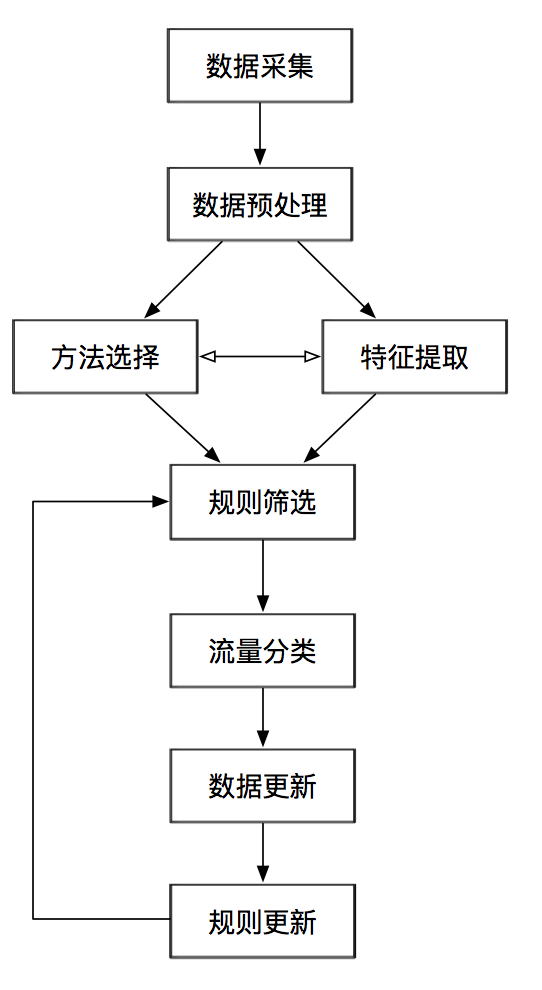
\includegraphics[scale=0.3]{../../Figures/Procedure_of_Flow_Classification.png}
    \end{figure}
\end{frame}

\begin{frame}[fragile]
	\frametitle{主要工作}
	研究者的主要贡献有:
	\begin{itemize}
		\item \verb|数据收集|: 采集网络流量,并用传统方法进行了类别标定,形成了一个较为标准的数据集。
		\item \verb|特征提取|: 从流量数据中提取248种特征,并对其有效性进行了一定分析。这些特征在之后的研究中被广泛使用。
		\item \verb|算法改进|: 提出了一种改进的朴素贝叶斯算法,提高了分类准确率。
	\end{itemize}
%		\scriptsize
	%\begin{verbatim}
	   % \documentclass[handout,print,aspectratio=1610]{beamer}
	      %  ...
	    %\begin{document}
	      %  ...
	   % \end{document}
	%\end{verbatim}
\end{frame}

\begin{frame}[fragile]
	\frametitle{流量采集和特征提取}
	流量采集的方法:
	\begin{itemize}
		\item 使用网络监测系统进行流量收集,并进行人为标定。
		\item 为了降低数据偏向性,采取分时段采集的方法。
		\item 为验证算法的持续有效性,作者于一年后再次采集数据进行测试。
	\end{itemize}
	数据特征提取:
	\begin{itemize}
	    \item 特征的提取只需要用到数据包的头部信息。
	    \item 其中包含了数据中原有特征以及通过复杂计算所得的特征。
	\end{itemize}
\end{frame}

\begin{frame}[fragile]
	\frametitle{朴素贝叶斯算法}
	朴素贝叶斯算法是一种较为简单的机器学习算法,其优势在于计算速度。\\
	\begin{theorem}
	    定义:
		\begin{enumerate}
			\item 假设数据可分为k类,$C = \{c_1, c_2, ... , c_k\}$为数据中所有类别的集合,对任意的$c_j \in C$其中样本所占比例为$p(c_j)$。
			\item 对某个样本y,和某类别$c_j$,假设在此类别中出现该样本的概率为$f(y|c_j)$。
		\end{enumerate}
		那么根据贝叶斯公式,该样本属于$c_j$的概率为:
        $$p(c_j|y) = \frac{p(c_j)f(y|c_j)}{\sum _ {c_j} p(c_j) f(y|c_j)}$$
        其中$f(y|c_j)$称为y的先验概率,也可称为算法的核函数,可结合某些假设,根据数据自身的分布计算得出。常用的核函数有线性核、高斯核等。
	\end{theorem}
\end{frame}

\begin{frame}[fragile]
	\frametitle{改进的朴素贝叶斯算法}
	    作者将原有核函数改进为:
	    $$\hat{f}(t|c_j) = \frac{1}{n_{c_j}h}\sum_{x_i : C(x_i) = c_j} K(\frac{t-x_i}{h})$$
	    其中h,t均为引入的参数,K满足$\int_{-\infty}^{+\infty}K(t)dt = 1$,$n_{c_j}$为类别$c_j$中所有样本的个数。\\
	    之后作者使用FCBF算法,对数据的特征进行了筛选,并以准确率为评价指标,将分类结果与原始的朴素贝叶斯算法进行了对比,使用的工具为Weka数据挖掘平台。
	    
\end{frame}

\begin{frame}
    \frametitle{总结分析}
    该论文工作内容较为全面,基本覆盖了流量分析的全部内容,但仍存在一定不足:
    \begin{itemize}
        \item 朴素贝叶斯算法本身存在一定的局限性,对数据的分析结果未必适用于其它网络环境。
        \item 算法仍需改进,作者所收集的数据中,有某一类别占据了很大比例,使得整体准确率偏高,而根据结果可看出该算法对于其他类别的识别效果较差。
        \item 未对其它算法进行分析对比。
    \end{itemize}
\end{frame}

\begin{frame}
    \frametitle{研究点总结}
    根据本文,可大致总结以下研究点:
    \begin{enumerate}
        \item 机器学习算法本身的优化改进,或尝试算法之间的结合。
        \item 特征优化算法的改进,或相互结合。
        \item 针对对数据本身存在问题进行改进。
        \item 解决算法的自动更新问题,使其保持长期有效。
        \item 研究流量发生初期的分类,从而提高检测的及时性。
    \end{enumerate}
\end{frame}
\begin{frame}
    谢谢,敬请批评指正!
\end{frame}
\end{document}
